\documentclass{exam} 
\usepackage[T1]{fontenc}
\usepackage{pslatex}
 \usepackage[pdftex]{color}  
 \usepackage[pdftex]{graphicx}     
\usepackage{verbatim}
\usepackage{xcolor}
\usepackage{paralist}

\usepackage[colorlinks=true,urlcolor=red]{hyperref}
\setlength{\topmargin}{-0.5in}                  % topmargin now at 1in
\setlength{\textheight}{9.5in}                  % body of text = 9.5in
\setlength{\oddsidemargin}{0in}                 % left margin = 1.0in on odd-numbered pages
\setlength{\evensidemargin}{0in}                % left margin = 1.0in on even-numbered pages 
\setlength{\textwidth}{6.5in}                   % width of text line.
\setlength{\parindent}{0.0in}
\newcommand{\code}{\texttt}

\usepackage{listings}
\lstset{%
	language=Java,
	basicstyle=\footnotesize\ttfamily,
	numbers=left,
	numberstyle=\tiny,        
	xleftmargin=17pt,
        xrightmargin=5pt,
	frame=single,
	breaklines=true
}

\lstdefinestyle{buggy}{
  language=Java,
  emptylines=1,
  breaklines=true,
  basicstyle=\ttfamily\color{black},
  moredelim=**[is][\color{red}]{@}{@},
}

\lstdefinestyle{correct}{
  language=Java,
  emptylines=1,
  breaklines=true,
  basicstyle=\ttfamily\color{black},
  moredelim=**[is][\color{blue}]{@}{@},
}

\begin{document}

\definecolor{aquamarine}{rgb}{0,0,0.7}
\definecolor{blue}{rgb}{0,0,0.7}
\definecolor{red}{rgb}{1,0,0}

%
\vspace{0.2in}
\begin{center}
        {\large  %MACQUARIE UNIVERSITY\\
%\medskip
\includegraphics[scale=0.3]{../../logo.png}\\
\medskip
        {\it  Faculty of Science and Engineering\\}
        \vspace{0.2in}
         {\bf COMP125 Fundamentals of Computer Science\\
        Workshop Week 3\\}}
\end{center}
\vspace{0.3in}
%

%\renewcommand{\labelenumi}{\arabic{enumi}.}
\renewcommand{\labelenumi}{\alph{enumi}.}
 
\section*{Learning outcomes}

By the end of this session, you will know some of Java basics.
In particular, you will be able to design and write simple Java classes.

\section*{Questions}

\begin{questions}

\question {\bf Import-Export}\\
 
It is important to know how to import Java projects from archive files (.jar/ .zip) and how to export your project(s) into archive files. First. we'll learn how to import a project.

\begin{enumerate}
\item Click ``File" --> ``Import" --> ``Existing Projects into Workspace"
\item Select option ``Select Archive file" and click on ``Browse"
\item Choose the archive files (``.zip") that contains project(s) you want to open. Please note an archive file may contain multiple projects and click ``ok"
\item Check all projects you want to import and click ``Finish"
\end{enumerate}

Practice the above procedure using file \texttt{classesAndObjectsProgram.zip} file uploaded on iLearn under Section 3. You should see a project \texttt{classesObjectsProject} if correctly imported.

Next, we'll learn how to export a project.

\begin{enumerate}
\item Click ``File" --> ``Export" --> ``General" --> ``Archive file"
\item Select all projects you want to export in the archive file in the left panel
\item In the ``To archive file" section, choose file path and name and click ``Finish"
\end{enumerate}

Export the project \texttt{classesObjectsProject} to an archive file \texttt{<studentID>.zip} where <studentID> is your Student ID.

\question (Problem solving and loops) Write a function (or method) that when passed an integer, returns the number of times it has to be divided by two, to reach zero. For example, 19 (or -19) needs to be divided by two, five times, to reach zero. 

\begin{enumerate}
\item 19/2 = 9, 
\item 9/2 = 4, 
\item 4/2 = 2, 
\item 2/2 = 1, 
\item 1/2 = 0
\end{enumerate}

\begin{solution}
\begin{lstlisting}
public static int countDivisonsByTwo(int an) {
	int count = 0;
	while(n != 0) {
		count++;
		n/=2;
	}
	return count;
}
\end{lstlisting}
\end{solution}

\newpage

\question Design classes (no implementation) that encapsulate the following real life entities. Add up to three data members for each class. Select the three most important attributes if you think a class has more than three attributes. Describe your design in terms of a UML class diagram as shown in week 2 lecture.

\begin{enumerate}
\item Person
\item Cylinder
\item Book
\end{enumerate}

\begin{solution}
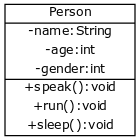
\includegraphics[width=5cm]{Person.png}
\vskip 0.5cm
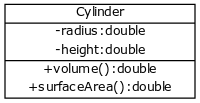
\includegraphics[width=5cm]{Cylinder.png}
\vskip 0.5cm
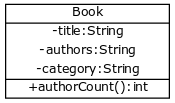
\includegraphics[width=5cm]{Book.png}
\vskip 0.5cm
\end{solution}

\question 

\begin{parts}

\part Consider the following class definition,

\begin{lstlisting}
public class Car {
	public String model;
	public int price;
}
\end{lstlisting}

Declare and instantiate an object \texttt{myCar} of class \texttt{Car}. Assign the value \texttt{Corolla} to the data member \texttt{model} and the value $21999$ to the data member \texttt{price} of object \texttt{myCar}.

\begin{solution}
\begin{lstlisting}
Car myCar = new Car();
myCar.model = ``Corolla'';
myCar.price = 21999;
\end{lstlisting}
\end{solution}

\part Consider the following class definition,

\begin{lstlisting}
public class Date {
	public int day, month, year;
}
\end{lstlisting}

Declare and instantiate an object \texttt{graduation} of class \texttt{Date}. Assign values to data members of object \texttt{graduation} such that it represents the date 13th April, 2011.

\begin{solution}
\begin{lstlisting}
Date graduation = new Date();
graduation.day = 13;
graduation.month = 4;
graduation.year = 2011;
\end{lstlisting}
\end{solution}

\end{parts}

\question 

\begin{parts}

\part Consider the following class definition,

\begin{lstlisting}[frame=single,style=buggy]
public class Time {
	@public@ int hour, minute, second;
}
\end{lstlisting}

Explain why it's a bad idea for the data members to be public, by writing a client that is malicious and assigns invalid values to the daa members of \texttt{Time} object.

\begin{solution}
\begin{lstlisting}
Time myTime = new Time();
time.hour = 888;
time.minute = -54;
time.second = -1729;
\end{lstlisting}
\end{solution}

\part Solve the problem of \texttt{public} data members in the previous part by first changing visibility of the data members of class \texttt{Time} to \texttt{private} and then adding getters and setters. The setter for \texttt{hour} should constrain the passed value in the range [0, 23]. That is, if the passed value is less than 0, \texttt{hour} should be 0, otherwise if the passed value is more than 23, \texttt{hour} should be 23, otherwise \texttt{hour} should become the passed value. Similarly, the setters for \texttt{minute} and \texttt{second} should constrain the passed value in the range [0, 59].

\begin{solution}
\begin{lstlisting}
public class Time {
	private int hour, minute, second;

	//setters
	public void setHour(int hour)  {
		if(hour >= 0 && hour <=23)
			this.hour = hour;
		else
			this.hour = 0;
	}

	public void setMinute(int minute)  {
		if(minute >= 0 && minute <=59)
			this.minute = minute;
		else 
			this.minute = 0;
	}

	public void setSecond(int second) {
		if(second >= 0 && second <=59)
			this.second = second;
		else 
			this.second = 0;
	}
	
	//getters
	public int getHour() {
		return hour;
	}

	public int getMinute() {
		return minute;
	}

	public int getSecond() {
		return second;
	}
}
\end{lstlisting}
\end{solution}

\part Declare, instantiate an object \texttt{t1} of class \texttt{Time} written in the previous part. Assign values to the data members such that it represents the time 19:30:45 (half past seven in the evening and another 45 seconds).

\begin{solution}
\begin{lstlisting}
Time t1 = new Time();
t1.setHour(19);
t1.setMinute(30);
t1.setSecond(45);
\end{lstlisting}
\end{solution}

\part Declare and instantiate an object \texttt{t2} of class \texttt{Time} written in the previous part. Assign 95 to \texttt{hour}, -78 to minute, and 55 to second. Display all data members on the console. What time would \texttt{t2} represent?

\begin{solution}
\begin{lstlisting}
Time t2 = new Time();
t2.setHour(95);
t2.setMinute(-78);
yourTime.setSecond(55);
System.out.println(t2.getHour()); //23
System.out.println(t2.getMinute()); //0
System.out.println(t2.getSecond()); //55
\end{lstlisting}
\end{solution}

\part List the mistakes (syntactical and logical) in the following constructor for class \texttt{Time} - 

\begin{lstlisting}
public void time(int h) {
	hour = h;
	minute = 0;
	second = 0;
}
\end{lstlisting}

\begin{solution}
\begin{itemize}
\item Constructor has no return type
\item Name of constructor should be \textbf{exactly} the same as the class name.
\item Constructor should use setters to assign values to data members.
\end{itemize}

Fixed constructor,

\begin{lstlisting}
public Time(int h) {
	setHour(0);
	setMinute(0);
	setSecond(0);
}
\end{lstlisting}
\end{solution}

\part Add two constructors to class \texttt{Time} with the following requirements:

\begin{itemize}
\item A constructor that is passed three parameters, one for each data member.
\item A constructor that is passed two parameters, for hour and minute, and sets seconds to 0.
\end{itemize}

\begin{solution}
\begin{lstlisting}
public Time(int h, int m, int s) {
	setHour(h);
	setMinute(m);
	setSecond(s);
}

public Time(int h, int m, int s) {
	setHour(h);
	setMinute(m);
	setSecond(0); //default value
}
\end{lstlisting}
\end{solution}

\part Assuming the two constructors have been added to class \texttt{Time} according to previous part. Will the following program run successfully, or result in a compilation error? Explain your answer. Also, if there is a compilation error, what should be done to fix it?

\begin{lstlisting}
Time ourTime = new Time();
\end{lstlisting}

\begin{solution}
It will result in a compilation error, since once parameterized constructors are defined, Java expects us to define the default constructor as well, and the default constructor that Java provides is no longer valid. The solution, therefore, is to add a default constructor.

\begin{lstlisting}
public Time() {
	setHour(0);
	setMinute(0);
	setSecond(0);
}
\end{lstlisting}
\end{solution}
\end{parts}
\question {\bf Assessed exercise}\\

\begin{enumerate}
\item Write a class definition for a \texttt{Line} in the first quadrant, as represented by its end points $(x_1, y_1)$ and $(x_2, y_2)$ such that $x_1, y_1, x_2, y_2 \geq 0$. It should include,

\begin{enumerate}
\item Correct class header.
\item Data members with appropriate visibility and data types.
\item Getters
\item Setters
\item Constructors
	\begin{enumerate}
		\item With no parameters. First and second points should be $(0, 0)$.
		\item With two parameters for $(x_1, y_1)$. Second point should be $(0, 0)$.
		\item With four parameters for $(x_1, y_1), (x_2, y_2)$.
	\end{enumerate}
\item A method \texttt{getLength()} that returns the length of the line as computed by the pythagorean formula 
\vskip 0.5cm
$d = \sqrt{(x_2 - x_1)^2 + (y_2 - y_1)^2}$.

You can compute square root of a numerical value $val$ by using \texttt{Math.sqrt(val)}.

\item The method \texttt{toString()} that returns the \texttt{String} representation of object of class \texttt{Line}. For example, if a line goes from (1.5, 2.5) to (8, 6.5), the method should return \texttt{``(1.5, 2.5) to (8, 6.5)''}.
\end{enumerate}

\item Write a piece of client code that -

\begin{enumerate}
\item Declare and instantiate an object \texttt{myLine} of class \texttt{Line} that represents a line from (4.2, 3.5) to ((6.5, 1.2)
\item Display the details of the object \texttt{myLine}. Which method is used? Do you call that method explicitly?
\item Store the length of \texttt{myLine} in variable \texttt{myLength} and display it on the console.
\item Change one of the end-points of the line from the previous coordinate of (4.2, 3.5) to a new coordinate (1.5, 7.5), and display the details of the line once more.
\end{enumerate}
\end{enumerate}

\begin{solution}
\newpage
\begin{lstlisting}
public class Line {
	private double x1, y1, x2, y2;

	public double getX1() {
		return x1;
	}

	public void setX1(double x1) {
		this.x1 = Math.abs(x1);
	}

	public double getY1() {
		return y1;
	}

	public void setY1(double y1) {
		this.y1 = Math.abs(y1);
	}

	public double getX2() {
		return x2;
	}

	public void setX2(double x2) {
		this.x2 = Math.abs(x2);
	}

	public double getY2() {
		return y2;
	}

	public void setY2(double y2) {
		this.y2 = Math.abs(y2);
	}

	public Line() {
		setX1(0);
		setY1(0);
		setX2(0);
		setY2(0);
	}
	
	public Line(double x1, double y1) {
		setX1(x1);
		setY1(y1);
		setX2(0);
		setY2(0);
	}
	
	public Line(double x1, double y1, double x2, double y2) {
		setX1(x1);
		setY1(y1);
		setX2(x2);
		setY2(y2);
	}
	
	public double getLength() {
		return Math.sqrt(Math.pow(x2-x1, 2) + Math.pow(y2-y1, 2));
	}
	
	public String toString() {
		return ``(''+x1+``,''+y1+``) to (''+x2+``, ''+y2+``)'';
	}
}
\end{lstlisting}
\end{solution}

\begin{solution}
\begin{lstlisting}
public class Client {
	public static void main(String[] args) {
		Line myLine = new Line(4.2, 3.5, 6.5, 1.2);
		System.out.println(myLine); //displays details using toString()
		double myLength = myLine.getLength();
		System.out.println(myLength);
		myLine.setX1(1.5);
		myLine.setY1(7.5);
		System.out.println(myLine); //displays details using toString()
	}
}		
\end{lstlisting}
\end{solution}

\end{questions}


\end{document}
